\chapter{Adaptive Filtering}

The previous chapter on wireless channel modeling established %
the wireless channel as a type of FIR filter. The aim of the %
receiver is to undo the effects of the channel filter. %
Figure \ref{fig:CommSysModel}. shows the communications %
system model as described in \cite{Sklar01}, for this section %
we'll draw our attention to the section of the model beginning %
at pulse modulation and ending at detection. 

\begin{figure}[h!]
	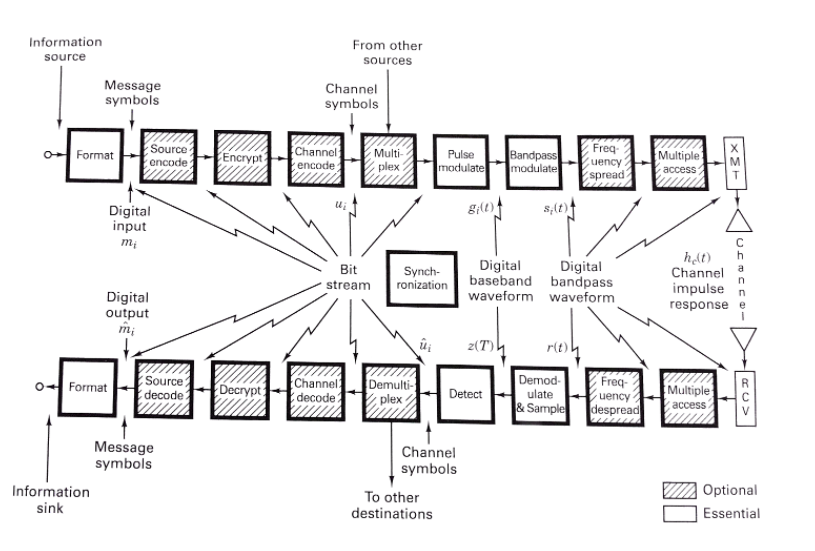
\includegraphics[width=\linewidth]{./Figures/Adaptive%
		Filters/CommunicationsSystemModel.png}
	\caption{Communications System Model \cite{Sklar01}}
	\label{fig:CommSysModel}
\end{figure}

The wireless system transfer function can be defined as:

\begin{align}
	H(f) = H_{t}(f)H_{c}(f)H_{r}(f)
\end{align}

where $H_{t}$ is the transfer function of the transmit filter, 
defined in the pulse modulate block, %
$H_{c}(f)$ is the transfer function of the channel, and $H_{r}%
(f)$ is the transfer function of the receive filter, defined in %
the demodulate and sample block. It's clear from this %
expression that the received baseband symbols at the %
detect block will be distorted by the channel filter $H_{c}%
(f)$, the goal of equalisation is to define an equalisation %
transfer function $H_{e}(f)$ that removes the effect of %
the channel filter. Such that the new system transfer %
function looks like this:

\begin{align}
	H(f) = H_{t}(f)H_{c}(f)H_{r}(f)H_{e}(f)
\end{align}

where

\begin{align}
	H_{c}(f)H_{e}(f) = 1
\end{align}



%TODO: insert diagram of the channel filter followed by
% an equalising filter

%TODO: provide a mathematical description of this equalisation
% effect

Throughout this entire chapter my development of adaptive filters %
will quite closely follow \cite{Hay02}. I'll start by %
developing the zero-forcing solution and the minimum mean square %
error solution also known as the Wiener solution. I'll then develop %
the stochastic gradient and the least mean square solution. A brief %
development of the recursive least square will be covered here as %
well.

\section{A Static Filter and The Wiener Solution}

%TODO: develop the Zero-forcing solution

%TODO: Develop the Wiener Solution

\section{Stochastic Gradient and the Least Mean Square}
\subsection{Normalised-Least Mean Square}

\section{Recursive Least Square}
\subsection{Kalman filters}  % Do I want to cover these?

